\documentclass[12pt]{article}
\usepackage[
  top=0.4cm,
  bottom=1.7cm,
  left=1.7cm,
  right=1.7cm,
  includehead,includefoot,
  heightrounded, % to avoid spurious underfull messages
]{geometry} 
\usepackage{wasysym} 
\usepackage{hyperref}

\usepackage{fancyhdr}
\fancyhf{} % clear all header and footers
\renewcommand{\headrulewidth}{0pt} % remove the header rule
\cfoot{\thepage}
\pagestyle{fancy}
\usepackage{wasysym} 
\usepackage{hyperref}
\usepackage{graphicx}
\usepackage{placeins}
\usepackage{epsfig}
\usepackage{epstopdf}
\usepackage{color}

\renewcommand{\familydefault}{\sfdefault}
\newcommand{\marker}[1]{Marker \color{red}\textbf{#1}\color{black}}

\title{\vspace{-1cm}\textbf{Dover War Memorial Project - User Guide}\vspace{-1cm}}
\date{}
\author{}
%%%%% document start
\begin{document}

\maketitle

This document acts as a user guide for someone who will be also performing administration functions (i.e. it's not for the general public). It will identify features of each page, and how to perform all the actions required to maintain and update the website. Buttons on screen are labelled in \textit{italics}, with text to be entered or displayed in \texttt{monospace}.

\tableofcontents
\newpage

\section{Navigation \& Login}
There are two main menu bars on the site. These are displayed on every single page, with the top bar gaining an extra row when logged in. The text disappears when viewed on mobile, for space reasons. The home page contains the same content as before, along with some dynamic data: a summary of the most recent news article and the names of any casualties that died on this day.

\subsection{What does the Home Page do?}
Figure~\ref{fig:home} shows the home page as viewed when not logged in. \marker{1}\ links back to the home page, \marker{2}\ navigates to the Latest News area (Section~\ref{sec:siteUpdate}), \marker{3}\ to the Casualty Index (Section~\ref{sec:casualtyIndex}), \marker{4}\ to the Articles area (Section~\ref{sec:articles}), \marker{5}\ the Search area (Section~\ref{sec:search}) and \marker{6}\ to the Contact Us page. At the bottom of the page, these links are reproduced, with the addition of \marker{7}, which navigates to the Login page (Section~\ref{ssec:login}). Other areas on the page are the latest news article (\marker{8}), the list of casualties who died today (\marker{9}) and the main narrative (\marker{10}).

\begin{figure}[h]
  \centering
 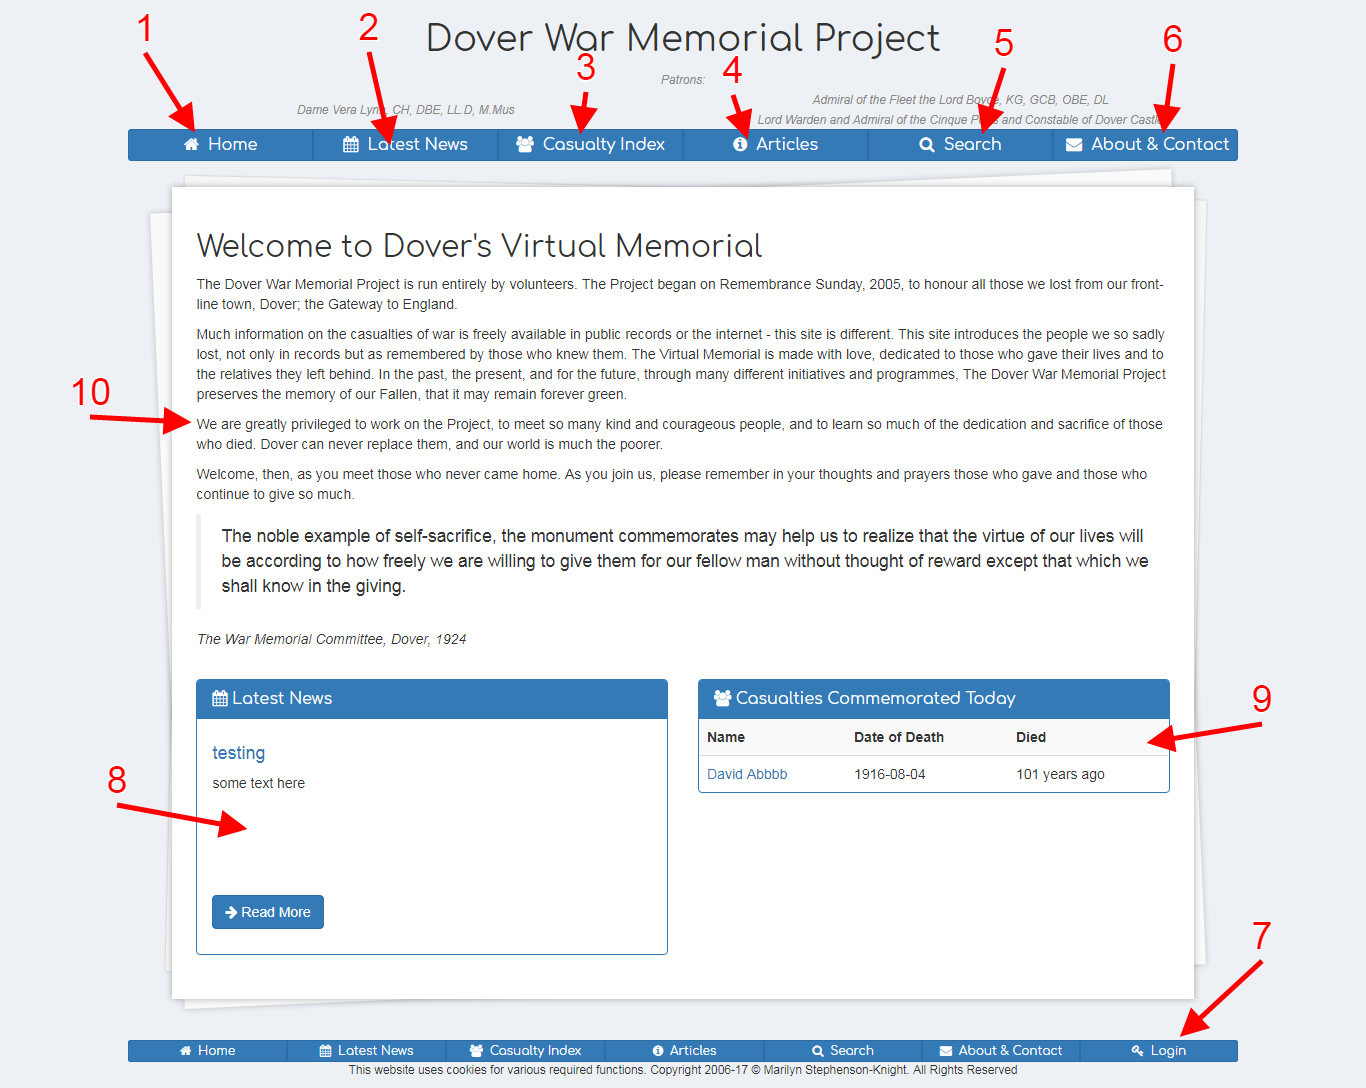
\includegraphics[width=.9\textwidth]{pics/home.png}
	\caption{Home Page}\label{fig:home}
\end{figure}

\newpage
\FloatBarrier
\subsection{How do I login?}\label{ssec:login}
To login, click the \textit{Login} button on the bottom menu bar (see \marker{7}\ on Figure~\ref{fig:home}). The login page is then loaded (Figure~\ref{fig:login}), which allows the user to login to the site to make various changes. \marker{1}\ is where the username must be entered with \marker{2}\ being the password field. \marker{3}\ submits this information.

\begin{figure}[h]
  \centering
 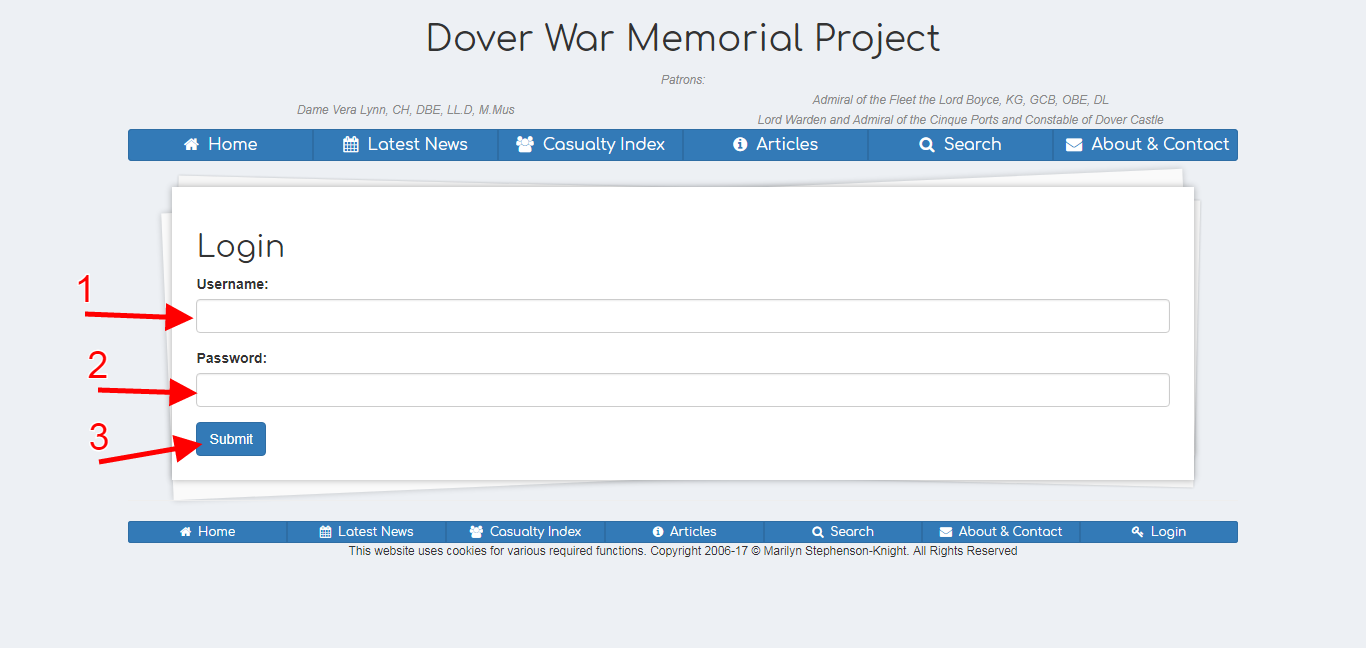
\includegraphics[width=.9\textwidth]{pics/login.png}
	\caption{Login Page}\label{fig:login}
\end{figure}

\newpage
\FloatBarrier
\subsection{How does the Home Page look after Login?}
Once a user has logged in, menu bars change. The top menu bar gains another row, with the login button on the bottom bar being replaced with a logout button, as can be seen in Figure~\ref{fig:home_login}. \marker{1}\ shows the currently logged in user, \marker{2}\ navigates to the config page (Section~\ref{sec:config}) and \marker{3}\ the admin help page (where this document is stored). \marker{4}\ and \marker{5}\ allow the user to logout. \marker{6} allows the user to edit the narrative text. These appear in numerous places across the site.

\begin{figure}[h]
  \centering
 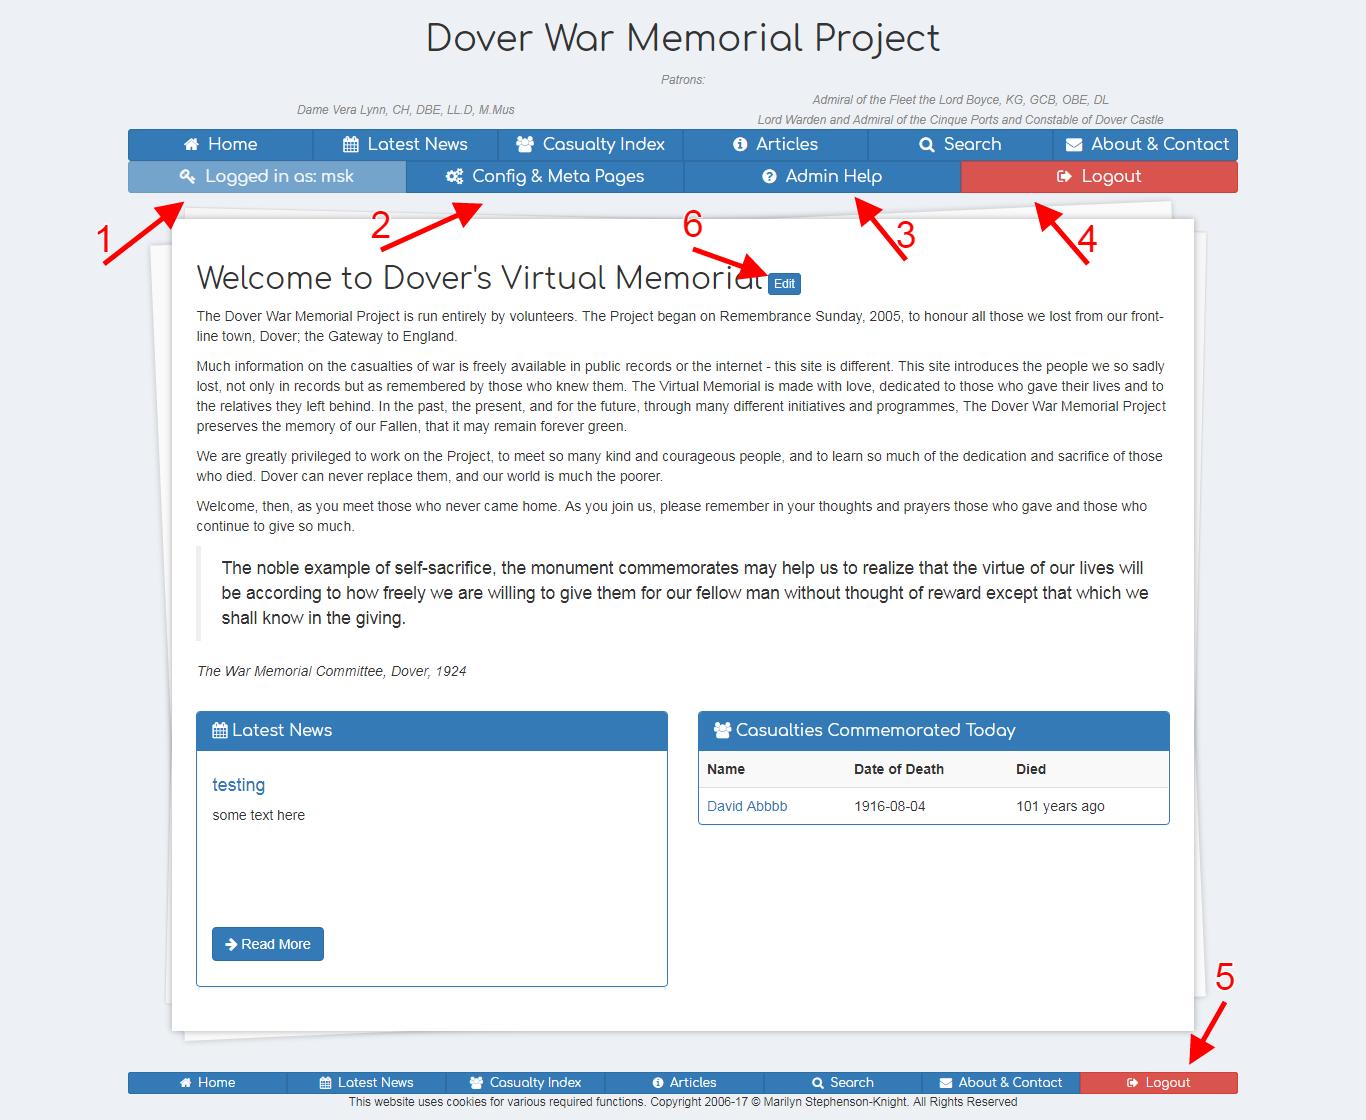
\includegraphics[width=.9\textwidth]{pics/home_login.png}
	\caption{Home Page after Login}\label{fig:home_login}
\end{figure}

\newpage
\FloatBarrier
\section{Site Updates}\label{sec:siteUpdate}
This section of the site contains two areas: Latest News, and a Change Log. The latest news section is for interesting updates and events that you may wish to bring attention to, in a similar way to the current latest news page. The most recent news article is also displayed on the home page.

The Change Log is a list of all the changes on the site (or rather, all the changes when you have entered a description of the change). This allows those visitors who wish to know what exactly is changing and when the ability to do so. It's also quite useful to show that the site is ``fresh'' and being regularly updates.

Navigate to Site Update section, by clicking the \textit{Latest News} link in either menu bar.

\subsection{How do I view a List of Updates?}
\subsection{How do I view a particular Update?}
\subsection{How do I Add or Edit an Update?}
\subsection{How do I delete an Update?}
\subsection{How do I view a List of Changes?}
\subsection{How do I delete an Change Log item?}

\section{Casualty Index}\label{sec:casualtyIndex}
casualties
\subsection{How do I view a List of all Memorials?}
\subsection{How do I view the Memorial Map?}
\subsection{How do I view a particular Memorial?}
\subsection{How do I Add or Edit a Memorial?}
\subsection{How do I delete a Memorial?}
\subsection{How do I view a Casualty?}
\subsection{How do I view a Casualty's Data?}
\subsection{How do I Add or Edit a Casualty?}
\subsection{How do I delete a Casualty?}


\section{Articles}\label{sec:articles}
articles
\subsection{How do I view the list of Articles?}
\subsection{How do I view a particular Article?}
\subsection{How do I Add or Edit an Article?}
\subsection{How do I delete an Article?}

\section{Search}\label{sec:search}
Search
\subsection{How do I perform a Text Search?}
\subsection{How do I perform a Data Search?}
\subsection{How do I view the Search Results?}

\section{Config \& Meta Pages}\label{sec:config}
Config
\subsection{How do I view the config page?}
\subsection{How do I view a list of Places?}
\subsection{How do I Add, Edit or Delete a Place?}
\subsection{How do I view a list of Ranks?}
\subsection{How do I Add, Edit or Delete a Rank?}
\subsection{How do I view a list of Regiment / Service?}
\subsection{How do I Add, Edit or Delete a Regiment / Service?}
\subsection{How do I view a list of Relation Types?}
\subsection{How do I Add, Edit or Delete a Relation Type?}
\subsection{How do I view a list of Service Country?}
\subsection{How do I Add, Edit or Delete a Service Country?}
\subsection{How do I view a list of Wars?}
\subsection{How do I Add, Edit or Delete a War?}
\subsection{How do I view a List of Recently Uploaded Casualties?}

\section{Others}
Others
\subsection{How do I use the Narrative Buttons?}

\end{document}